%% 
%% Copyright 2007-2019 Elsevier Ltd
%% 
%% This file is part of the 'Elsarticle Bundle'.
%% ---------------------------------------------
%% 
%% It may be distributed under the conditions of the LaTeX Project Public
%% License, either version 1.2 of this license or (at your option) any
%% later version.  The latest version of this license is in
%%    http://www.latex-project.org/lppl.txt
%% and version 1.2 or later is part of all distributions of LaTeX
%% version 1999/12/01 or later.
%% 
%% The list of all files belonging to the 'Elsarticle Bundle' is
%% given in the file `manifest.txt'.
%% 

%% Template article for Elsevier's document class `elsarticle'
%% with numbered style bibliographic references
%% SP 2008/03/01
%%
%% 
%%
%% $Id: elsarticle-template-num.tex 168 2019-02-25 07:15:41Z apu.v $
%%
%%
\documentclass[preprint,12pt]{elsarticle}

%% Use the option review to obtain double line spacing
%% \documentclass[authoryear,preprint,review,12pt]{elsarticle}

%% Use the options 1p,twocolumn; 3p; 3p,twocolumn; 5p; or 5p,twocolumn
%% for a journal layout:
%% \documentclass[final,1p,times]{elsarticle}
%% \documentclass[final,1p,times,twocolumn]{elsarticle}
%% \documentclass[final,3p,times]{elsarticle}
%% \documentclass[final,3p,times,twocolumn]{elsarticle}
%% \documentclass[final,5p,times]{elsarticle}
%% \documentclass[final,5p,times,twocolumn]{elsarticle}

%% For including figures, graphicx.sty has been loaded in
%% elsarticle.cls. If you prefer to use the old commands
%% please give \usepackage{epsfig}

%% The amssymb package provides various useful mathematical symbols
\usepackage{amssymb}
%% The amsthm package provides extended theorem environments
%% \usepackage{amsthm}

%% The lineno packages adds line numbers. Start line numbering with
%% \begin{linenumbers}, end it with \end{linenumbers}. Or switch it on
%% for the whole article with \linenumbers.
%% \usepackage{lineno}

\journal{journal X}

\begin{document}

\begin{frontmatter}

%% Title, authors and addresses

%% use the tnoteref command within \title for footnotes;
%% use the tnotetext command for theassociated footnote;
%% use the fnref command within \author or \address for footnotes;
%% use the fntext command for theassociated footnote;
%% use the corref command within \author for corresponding author footnotes;
%% use the cortext command for theassociated footnote;
%% use the ead command for the email address,
%% and the form \ead[url] for the home page:
%% \title{Title\tnoteref{label1}}
%% \tnotetext[label1]{}
%% \author{Name\corref{cor1}\fnref{label2}}
%% \ead{email address}
%% \ead[url]{home page}
%% \fntext[label2]{}
%% \cortext[cor1]{}
%% \address{Address\fnref{label3}}
%% \fntext[label3]{}

\title{Defects and welds detection and classification approach based on CNN for oil pipeline MFL data}

%% use optional labels to link authors explicitly to addresses:
%% \author[label1,label2]{}
%% \address[label1]{}
%% \address[label2]{}

\author{Iurii Katser, Viacheslav Kozitsin, Ivan Maksimov}

\address{Skolkovo Institute of Science and Technology}

\begin{abstract}
%% Text of abstract

\end{abstract}

%%Graphical abstract
%\begin{graphicalabstract}
%%\includegraphics{grabs}
%\end{graphicalabstract}

%%Research highlights
%\begin{highlights}
%	\item Research highlight 1
%	\item Research highlight 2
%\end{highlights}

\begin{keyword}
%% keywords here, in the form: keyword \sep keyword
deep learning \sep computer vision \sep convolutional neural networks \sep anomaly detection \sep fault detection \sep oil pipelines \sep defects \sep welds
%% PACS codes here, in the form: \PACS code \sep code

%% MSC codes here, in the form: \MSC code \sep code
%% or \MSC[2008] code \sep code (2000 is the default)

\end{keyword}

\end{frontmatter}

%% \linenumbers

%% main text
\section{INTRODUCTION}
\label{INTRODUCTION}
Anomaly detection problems have a great importance in industrial applications, because anomalies usually represent faults, failures or the emergence of such.
To detect these automatically, advanced analytic algorithms, including machine learning- and deep learning-based, can be applied.
In this work, we investigate deep neural network performances in providing hindsight in oil pipeline diagnostics.
This system spans over thousands of kilometers, which makes manual inspection very costly and sometimes impossible.
The damage of pipelines that transport petroleum and gas products lead to severe environmental problems.
Eliminating breakthroughs and their consequences is expensive.
To avoid accidents, it is recommended to improve diagnostics quality and to increase the frequency of in-line-inspection (ILI) tools deployment.
ILI tools, also referred to as pipeline inspection gauges (Fig.~\ref{ris:ili}), use Hall effect for measuring localized Magnetic Flux Leakage (MFL) intensity along the pipe wall. While moving along the pipe gauge inspects the wall and detects the magnetic field leaks. MFL technique is the most common approach for oil and gas pipelines nondestructive testing nowadays.
\begin{figure}[ht]
	\center{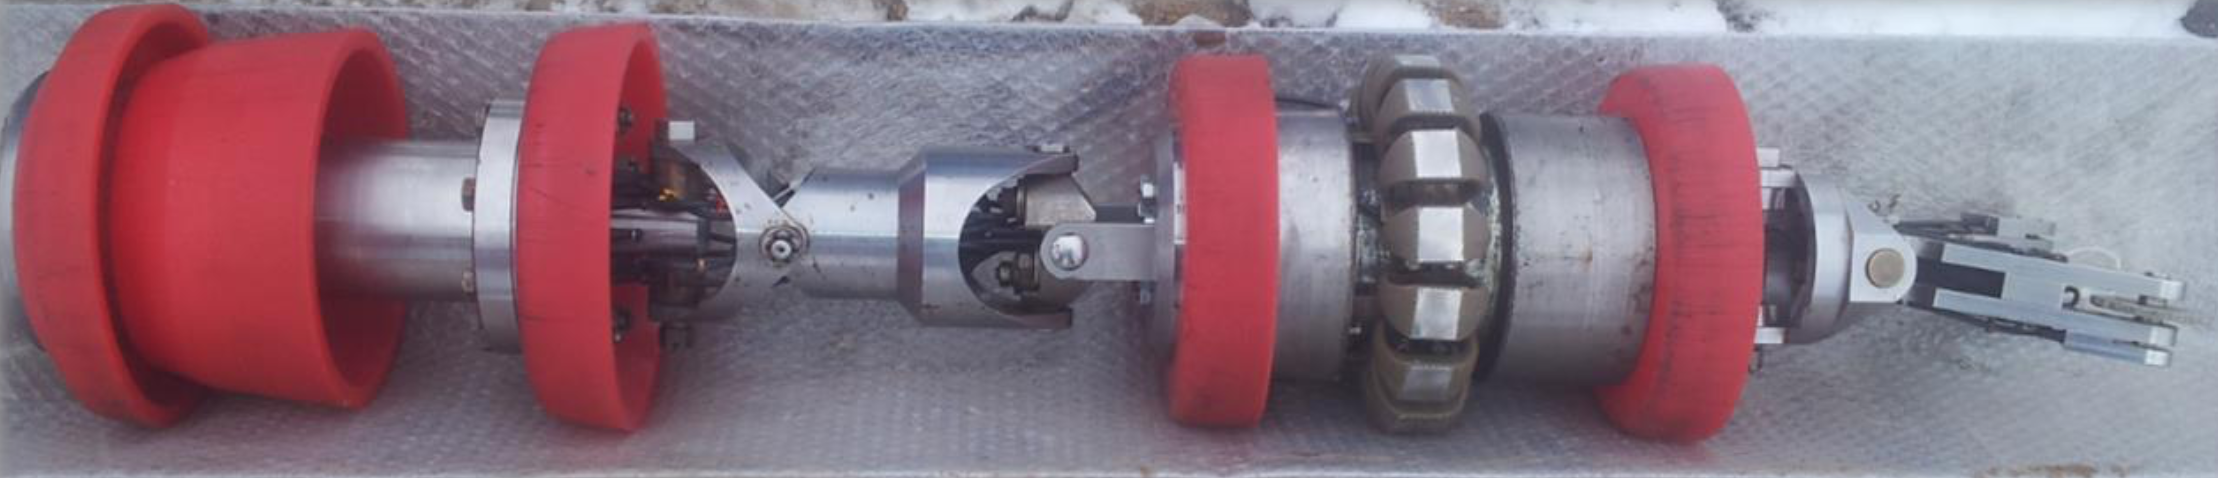
\includegraphics[scale=0.35]{pictures/ili.png}}
	\caption{In-line-inspection tool}
	\label{ris:ili}
\end{figure}
The data collected during the inspection can be further analyzed for main diagnostics problems solving: damage and defects detection, their localization, diagnosis or defects classification.
Analysis results are useful for assets managing and repair priorities determination.

There are three main classes of data that are attended to by diagnostics personnel.
They are presented in Fig.~\ref{ris:classes}.
Some other classes of data (pipe tee, bend) are out of the scope of this work just like different classes of defects.
\begin{figure}[ht]
	\center{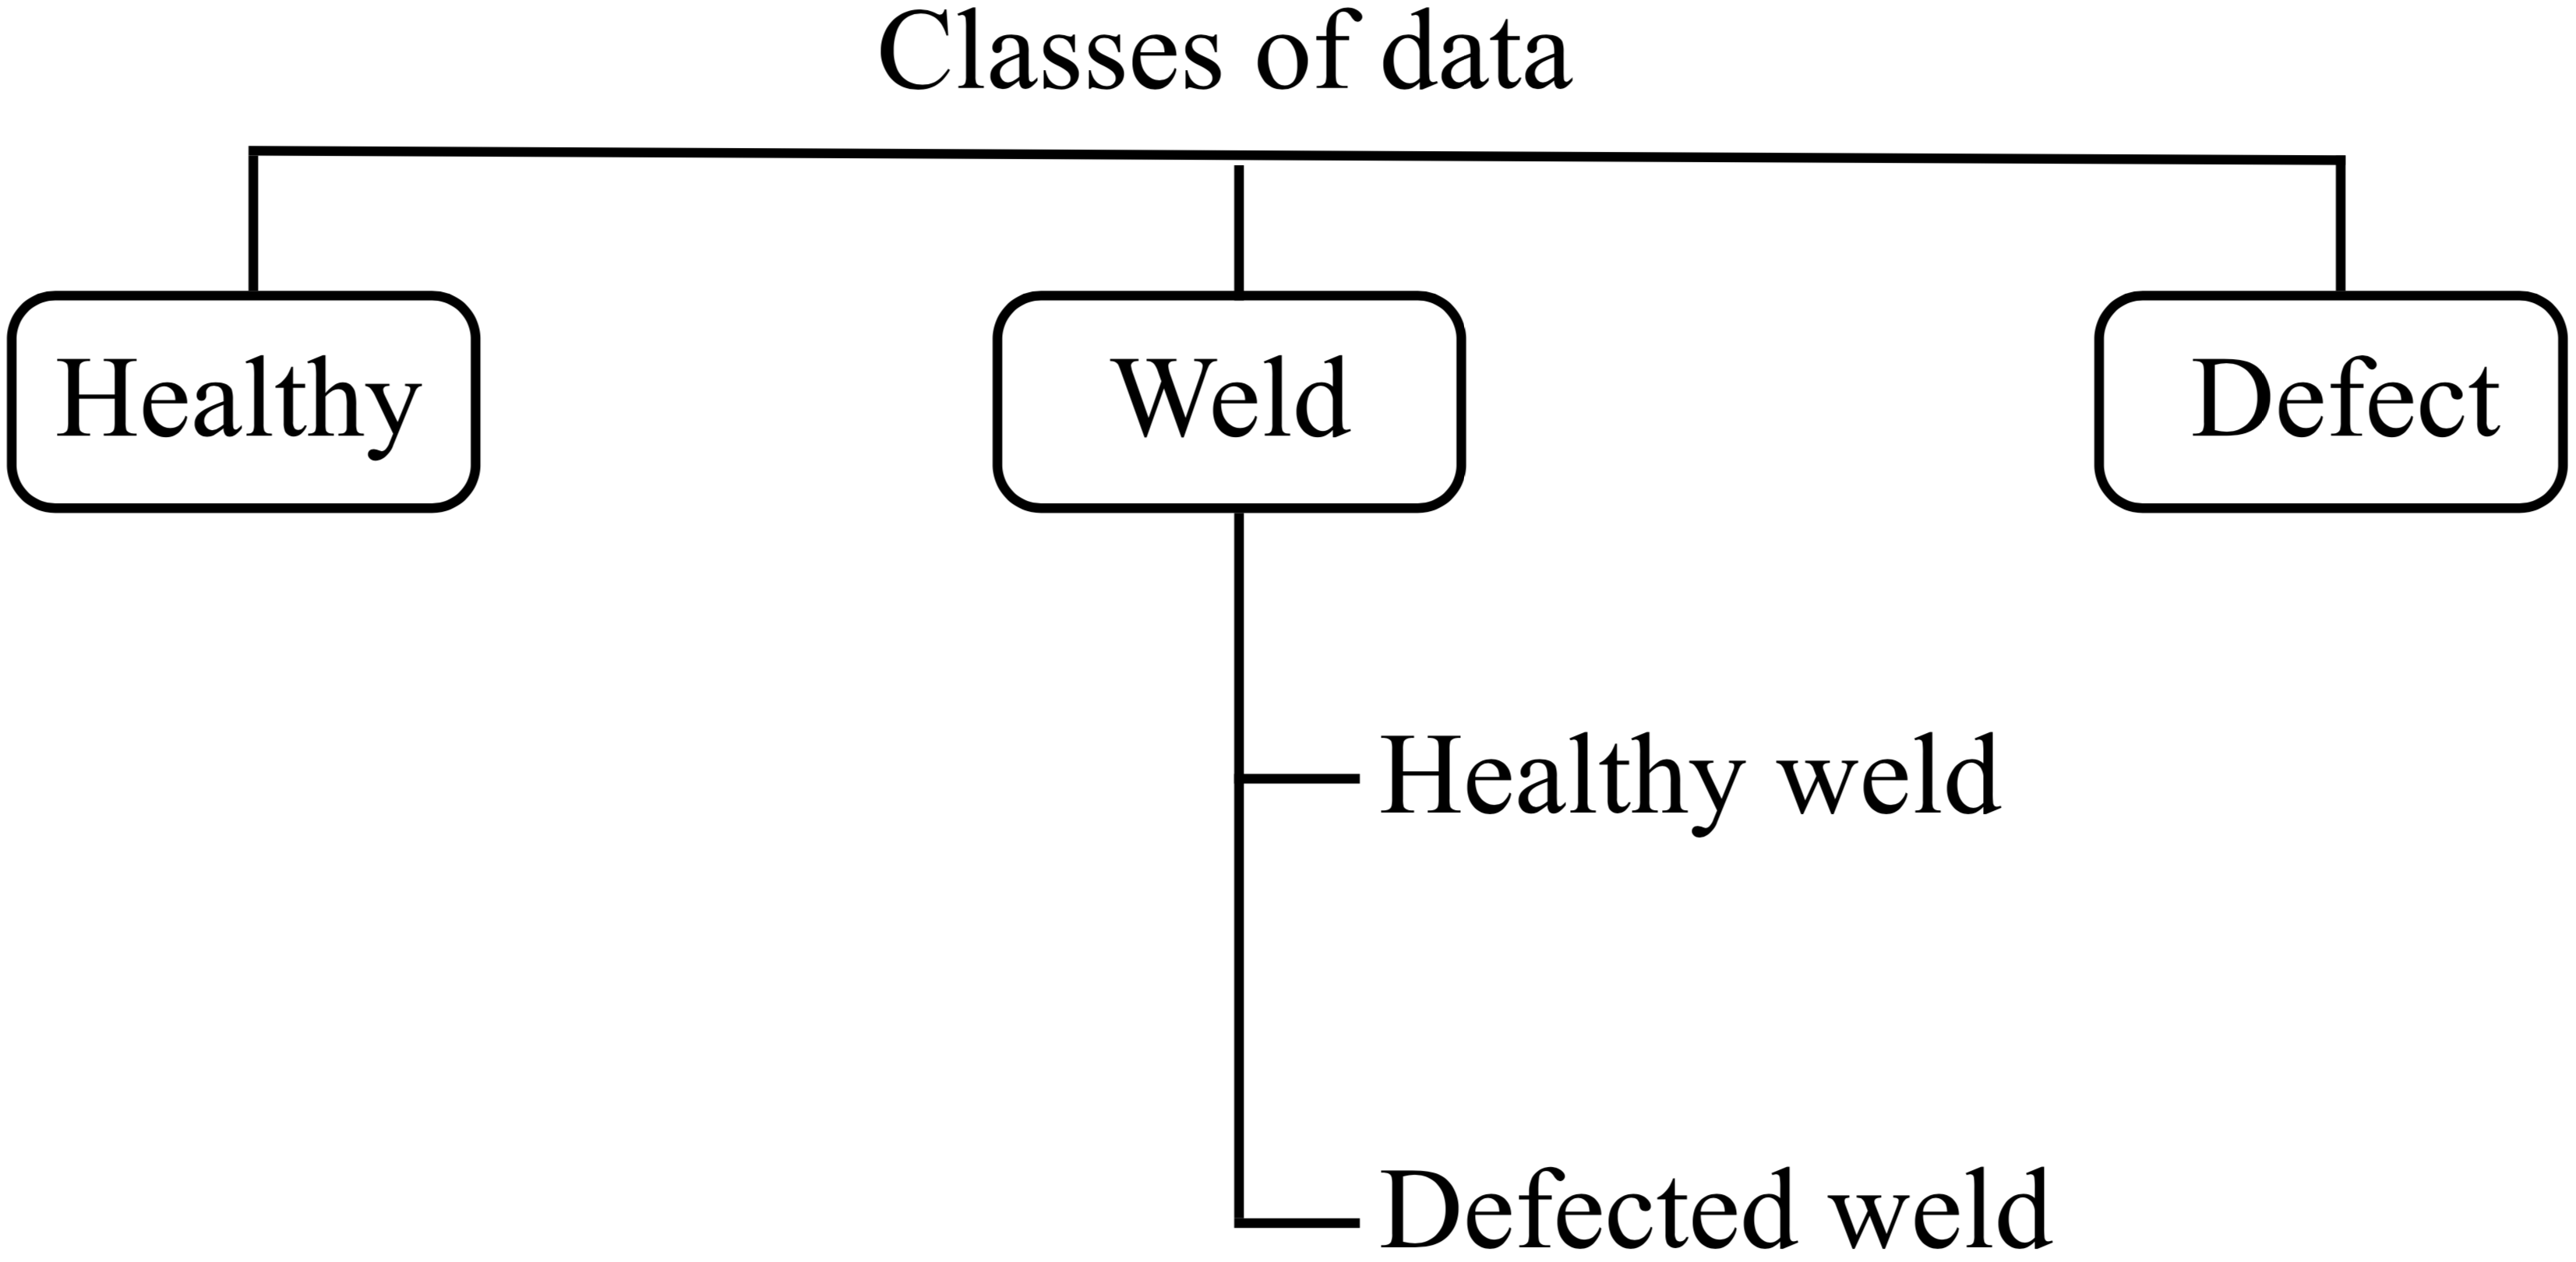
\includegraphics[scale=0.2]{pictures/classes.png}}
	\caption{Image classes that are distinguished in the work}
	\label{ris:classes}
\end{figure}

The rest of the paper is devoted to appraising computer vision (CV) techniques proficiency in oil pipeline diagnostics application.


\section{LITERATURE REVIEW}
\label{LITERATURE REVIEW}

\subsection{Pipelines defects diagnostics}

Magnetic Flux Leakage (MFL) technique is the most common approach for oil and gas pipelines nondestructive testing.
The data obtained during the pipeline inspection process is primarily analyzed by traditional machine learning (ML) methods.
A comparison of performance among different ML methods for defects identification problem is presented in \cite{Khodayari-Rostamabad2009}.
The main challenge for this approach is creating informative and important features that will be used as an input for ML methods.
Usually, these diagnostics features are generated using expert knowledge and manually-created heuristics.
It imposes the limitation on defects detection problem solving quality.
A variety of most successful features is presented and analyzed in details in \cite{Slesarev2017}.

Deep Learning showed significant progress and achieved incredible results in numerous applications, just in the past few years.
The image classification problem is one of the most successful applications of DL and Convolutional Neural Networks (CNNs) in particular.
To automate the process of feature generation in MFL data analysis, CNNs can be used either.
As an advantage, they can solve the defects or welds detection, classification and segmentation problems at the same time.
In literature there are examples of applying CNNs for defects detection \cite{Feng2017}, welds defect detection \cite{2020a}, welds and defects classification \cite{Yang2020}, defect size estimation \cite{Lu2019}.
For all mentioned applications, CNNs outperformed existing traditional approaches.
Nevertheless, still, there are just a few works dedicated to MFL data analysis using DL.
A number of particular problems that can be solved using a novel approach are not covered yet.
For instance, we could not find any works on applying CNNs to defects segmentation task, despite the importance of this problem solving according to \cite{Feng2017}.

In this work, we want to research two different problems:
\begin{enumerate}
	\item Defects detection (Picture classification task).
	\item Defects segmentation (Semantic segmentation task).
\end{enumerate}

For their solving, we propose CNNs of different architectures and compare their results with existing state-of-the-art approaches.
Moreover, we research different preprocessing techniques for dealing with typical issues in the MFL data.

\subsection{Unet}

asd \cite{Ronneberger2015a}

\section{DATASET DESCRIPTION AND PREPROCESSING PROCEDURES}
\label{DATASET DESCRIPTION AND PREPROCESSING PROCEDURES}
Although MFL data looks quite similar for different pipes and ILI tool types, it can differ significantly.
The data mainly depends on pipe size, wall width, sensors geometry, and other geometric characteristics.
Moreover, ILI tools differ a lot for different pipe sizes.
Therefore, the repeatability of the results for different datasets should be investigated additionally.
Following, we provide dataset characteristics, which are also presented in Table~\ref{tab:dataset}.
We have data collected from the 219 mm in diameter pipe.
MFL dataset provides information about a single inspection tool run.
Dataset has 64 features collected as an array with a constant step along with the ILI tool movement inside the pipe.
Dataset has 4470704 samples that represent 15162.85 meters long pipeline part.
Sample values vary from 0 to 4095 units.
It has 745 defects of different types and 1462 welds, 34 of which are defected.
Fig.~\ref{ris:defect_example} shows examples of healthy data, data with a weld, and with a defect.
Attached to the dataset technical report contains information about welds and defects location, defects types, sizes, and other related characteristics.
\begin{table}[!htb]
	\caption{Dataset characteristics.}
	\begin{center}
		\small
		\begin{tabular}{|  c | c   |}
			\hline
			Parameter & Value \\
			\hline
			Pipeline diameter, mm &  219 \\
			Pipeline length, m &  15162.85 \\
			Number of samples &  4470704 \\
			Number of features & 64 \\
			Min value & 0 \\
			Max value & 4095 \\
			Mean value &   \\
			Number of defects & 745 \\
			Number of welds (with defects) & 1462 (34) \\
			\hline
		\end{tabular}
		\label{tab:dataset}
	\end{center}
\end{table}

\begin{figure}[ht]
	\center{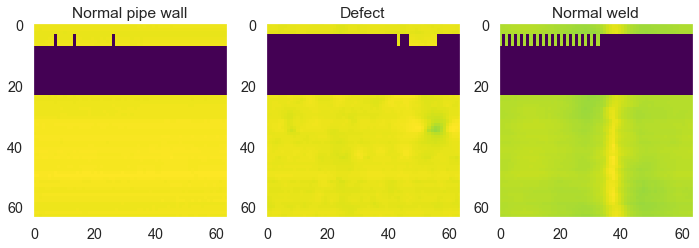
\includegraphics[scale=0.4]{pictures/1.png}}
	\caption{Example of the MFL data}
	\label{ris:defect_example}
\end{figure}

Raw data has several issues that don't allow us to solve CV problems without proper preprocessing.
They are:
\begin{enumerate}
	\item Sensors malfunctions (zeroed values cause bold horizontal line in Fig.~\ref{ris:defect_example});
	\item Displaced origins between data and reports coordinates;
	\item Inaccurate annotations, e.g., missed defects, wrong defect location, etc.
	\item No annotated data for the segmentation task.
\end{enumerate}

\subsubsection{Sensors malfunctions problem}
To deal with sensors malfunctions we suppose to fill the gaps (zeroed values) with values calculated by different methods.
Additionaly, we will consider values less than 2000 abnormal and replace them with zeroes during the preprocessing.
\begin{enumerate}
	\item Abnormal values are equal to 0. Then Min-Max scaling to $[0.5:1]$ range.
	\item Abnormal values are equal to the mean of normal values from one picture. Then Min-Max scaling.
	\item Abnormal values are equal to the mean of normal values over the column. Then Min-Max scaling.
	\item Abnormal values are equal to the mean of neighboring sensors over the column. Then Min-Max scaling.
	\item Abnormal values are equal to the interpolation results over the column. Then Min-Max scaling.
\end{enumerate}

The results of all applied methods are presented in Fig.~\ref{ris:filling_example}.
\begin{figure}[ht]
	\center{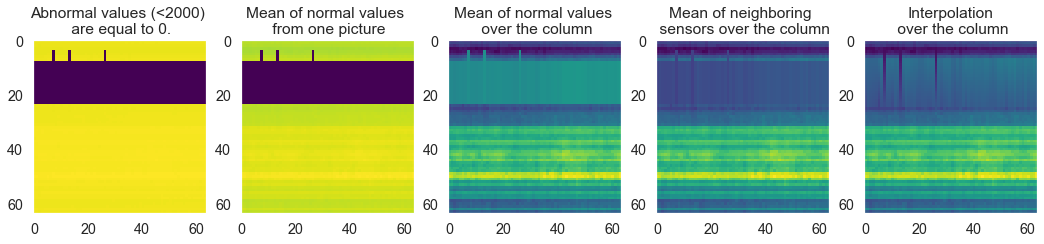
\includegraphics[scale=0.37]{pictures/2.png}}
	\caption{Comparison of methods for missing values filling}
	\label{ris:filling_example}
\end{figure}

Min-Max scaling can be applied using whole dataset or just one image.
Both approaches will be compared during the experiment conducting.

Since the ILI tool location data did not match the defect location data from the report, it was necessary to merge the data. The key factor here turned out to be that signal values from magnetic flux sensors grow at the weld site (Figure \ref{ris:prepr}). 

\begin{figure}[!h]
	\center{\includegraphics[width=0.82\linewidth]{pictures/prepr.png}}
	\caption{Location of a weld. The black vertical line is a weld, according to the report. Other lines are values from sensors.}
	\label{ris:prepr}
\end{figure}
The solution was to find the locations of the maxima of sensors data values and then to combine it with the weld coordinates.

\subsubsection{Inaccurate annotations problem}
This problem is a common one for oil and gas pipeline nondestructive testing \cite{Khodayari-Rostamabad2009}.
It appears to be a lot of missing defects that affect the quality of the problem.
Besides, there are wrong defect types and locations.
To eliminate wrong location issue, we additionaly searched extremums around the provided location and chose the defects or welds taking into account new coordinates.

\subsubsection{Augmentation}
Although we have a lot of data, we don't have a lot of defects and welds in comparison with healthy pipe wall instances.
We use the augmentation procedure to balance classes of pictures and increase the model's quality by increasing the number of pictures in small classes (defects, welds).
As an augmentation tool we use Albumentations library \cite{buslaev2020albumentations}.
All applied augmentations both for welds and defects are presented in Table~\ref{tab:aug}.
Applied augmentations details are presented in \cite{buslaev2020albumentations} and references therein.

\begin{table}[!htb]
	\caption{Applied augmentations.}
	\begin{center}
		\small
		\begin{tabular}{| c | c | c |}
			\hline
			Augmentation Type & Welds & Defects \\
			\hline
			Rotate90 &  - & \checkmark \\
			Rotate180 & \checkmark & \checkmark \\
			Rotate270 &  - & \checkmark \\
			VerticalFlip & \checkmark & \checkmark \\
			HorizontalFlip & \checkmark & \checkmark \\
			ElasticTransform & \checkmark & \checkmark \\
			GridDistortion & \checkmark & \checkmark \\
			OpticalDistortion & \checkmark & \checkmark \\
			Transpose & - & \checkmark \\
			RandomRotate90 &  - & \checkmark \\
			\hline
		\end{tabular}
		\label{tab:aug}
	\end{center}
\end{table}

Examples of augmentations are shown in Fig.~\ref{ris:aug_example}.
\begin{figure}[ht]
	\center{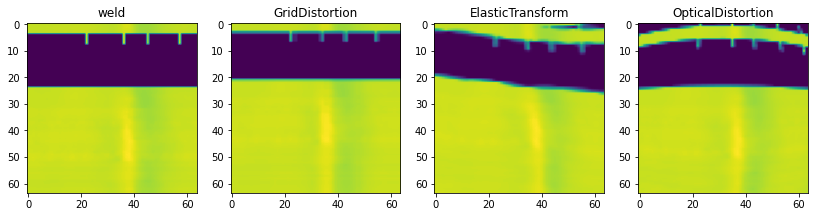
\includegraphics[scale=0.45]{pictures/4.png}}
	\caption{Examples of the augmented weld image}
	\label{ris:aug_example}
\end{figure}


The characteristics of the pipeline defects dataset are described in Table \ref{tab:alg1}.
\begin{table}[!htb]
	\caption{\label{tab:alg1}Dataset size for pipeline defects detection and segmentation problems}
	\begin{center}
		\small
		\begin{tabular}{| c | c  c  c |}
			\hline
			Data & Healthy & Defect & Weld \\
			\hline
			\multicolumn{4}{|c|}{Before augmentation}  \\
			\hline
			Train  & 11106 & 569 & 1130 \\
			Validation & 584 & 142 & 282 \\
			\hline
			\multicolumn{4}{|c|}{After augmentation}  \\
			\hline
			Train  & 11106 & 8535 & 11300 \\
			Validation & 584 & 142 & 282 \\
			\hline
		\end{tabular}
	\end{center}
\end{table}

\section{METHODS}
\label{METHODS}
Pipeline defect detection is composed of two problems. First, the defect should be detected, and further, it should be evaluated using segmentation results.
We propose here a novel CNN architecture for image classification.
Additionally, we present the existing architectures that achieve the best results in the MFL and X-ray data classification problems.

\subsection{CNN Preliminaries}

A CNN is a special type of a neural network that has proven  effective in computer vision applications. State-of-the-art results can be achieved in segmentation and classification tasks \cite{a10}. Compared to computer vision algorithms that do not take advantage of CNNs, much less pre-processing is required. More importantly, such networks are able to learn characteristics from data, which otherwise would have to be individually accounted for \cite{a11}.

Even though CNNs have been proposed in different architectures - to increase their efficiency for specific tasks and/or datasets, three different types of layers are used without exception, each with a specific propose: convolutional, pooling, and fully connected (linear) layers. The convolutional layers aim to extract feature maps of the input images by applying filters over different region of images. For instance, with $k$ filters, each filter having weight and bias of $w_i$ and $b_i$, respectively, the convolution of an image patch, $x_n$, can be written as follows:

\begin{equation}
f_{i,n}=\sigma(W_ix_n+b_i),
\end{equation}

where $\sigma$ is the activation function. Besides rectified linear units (ReLU), sigmoid or softmax activation functions, a multitude of different options exist, all having their individual advantages. These are applied on a layers's output neurons (e.g. after a convolutional layer).
After a number of convolutional layers, pooling layers are commonly applied in prominent network architectures to reduce the size of particular dimensions. Max-pooling and average-pooling are two examples. Pooling layers, alongside reducing dimensions's sizes, perform denoising when utilized on images. 
%Note, that max-pooling can execute denoising along with the dimensionality reduction task. 
% In the proposed CNN, presented in the next section, max-pooling is applied.
Fully connected layers are generally the last layers of CNNs, possessing a similar structure compared to the traditional neural networks\cite{a12}.

\subsection{CNN Structure}
%TODO merge two next paragraphs
%Performing fault detection on components is composed of two distinct problems that mussed be addressed. First, components of interest must be identified given an input image. Secondly, after successful segmentation of the respective component, its state must be classified (one of the modes of failure shown in Fig. \ref{fig:mof}). Even though a single network could be able to achieve this, a modular detection algorithm was developed, as depicted in  Fig. \ref{fig:structure}.
%Two distinct CNNs are used, one segmenting the components of interest and the second detecting faults. Utilizing two networks in serial, as shown, allows for easier implementation, as the segmentation and classification stage can be fine-tuned and trained individually. Furthermore, a modular system facilitates replacing components in the data-processing pipeline.
%

Proposed model (Fig.~\ref{ris:CNN_our}) consists of 5 Convolutional layers overall.
Each Convolutional layer is followed by BN and Dropout sequentially (not shown in Fig.~\ref{ris:CNN_our}).
All Convolutional layers have equal kernel size - 5 x 5.
All MaxPooling layers have equal kernel size - 2 x 2, and stride - 2.
From now on this CNN is marked as CNN-5.
\begin{figure}[ht]
	\center{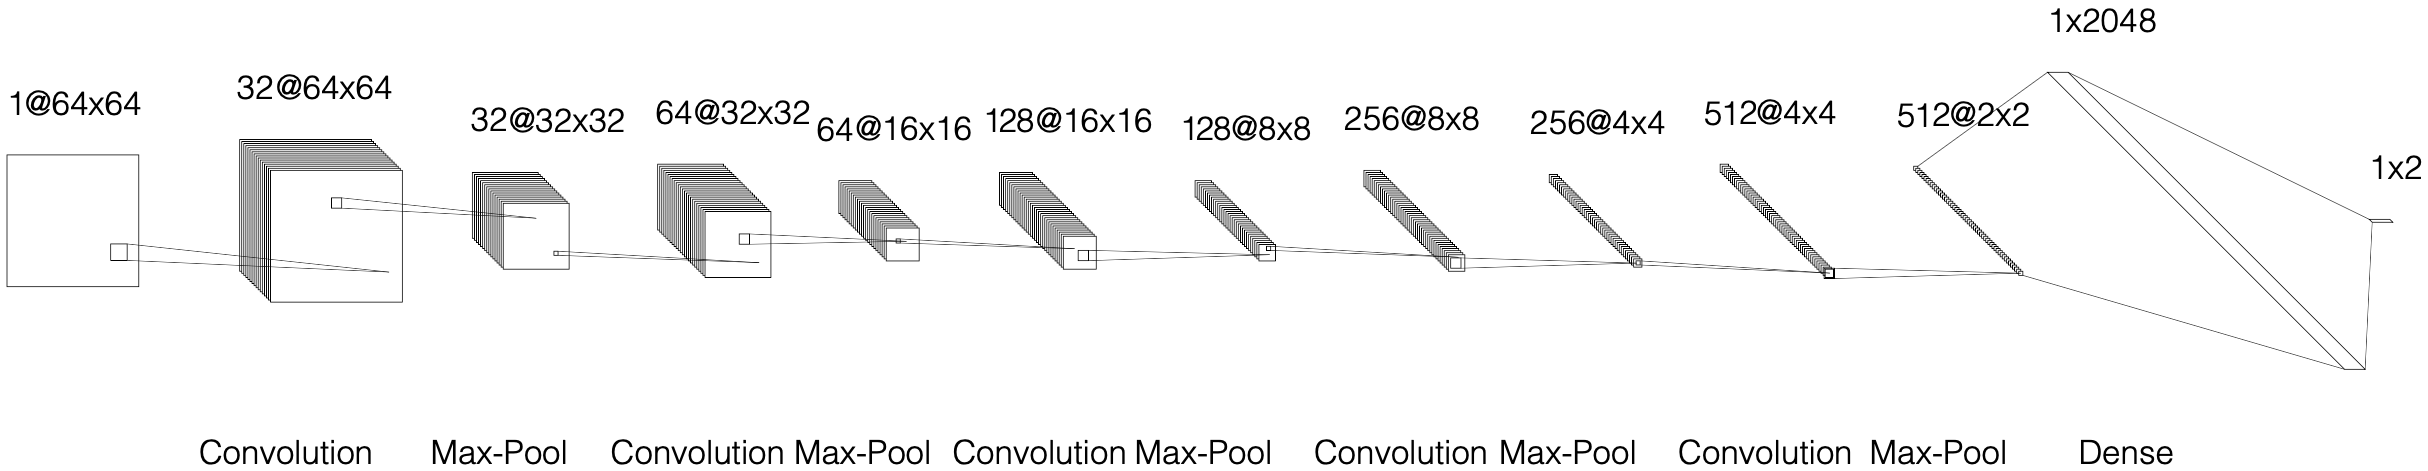
\includegraphics[scale=0.15]{pictures/CNN_our.png}}
	\caption{Architecture of the proposed CNN}
	\label{ris:CNN_our}
\end{figure}

\subsection{Performance metric}
For the classification problem we use Accuracy.
Accuracy is defined by the formula:
\begin{equation}
Acc = \frac{\sum_{i=0}^{N} 1_{\{\hat{y}_i=y_i\}}}{N}
\end{equation}
where $N$ - number of samples, $\hat{y}$ - predicted label, $y$ - true label.

\subsection{Loss functions}
Weighted Binary Cross-Entropy both for segmentation and detection problems:
\begin{equation}
wBCE =-\frac{1}{N} \sum_{i=1}^{N} w_{1} \cdot y_{i} \cdot \log \left(p\left(\hat{y_{i}}\right)\right)
+ w_{2} \cdot \left(1-y_{i}\right) \cdot \log \left(1-p\left(\hat{y_{i}}\right)\right)
\end{equation}

\subsection{Existing CNNs}

We reimplemented CNN from \cite{Feng2017} with one difference: we used squared pictures (64x64 pixels) as an input, so we didn't implement Normalization layer (first layer in the Fig.~\ref{ris:CNN_feng2017}).
\begin{figure}[ht]
	\center{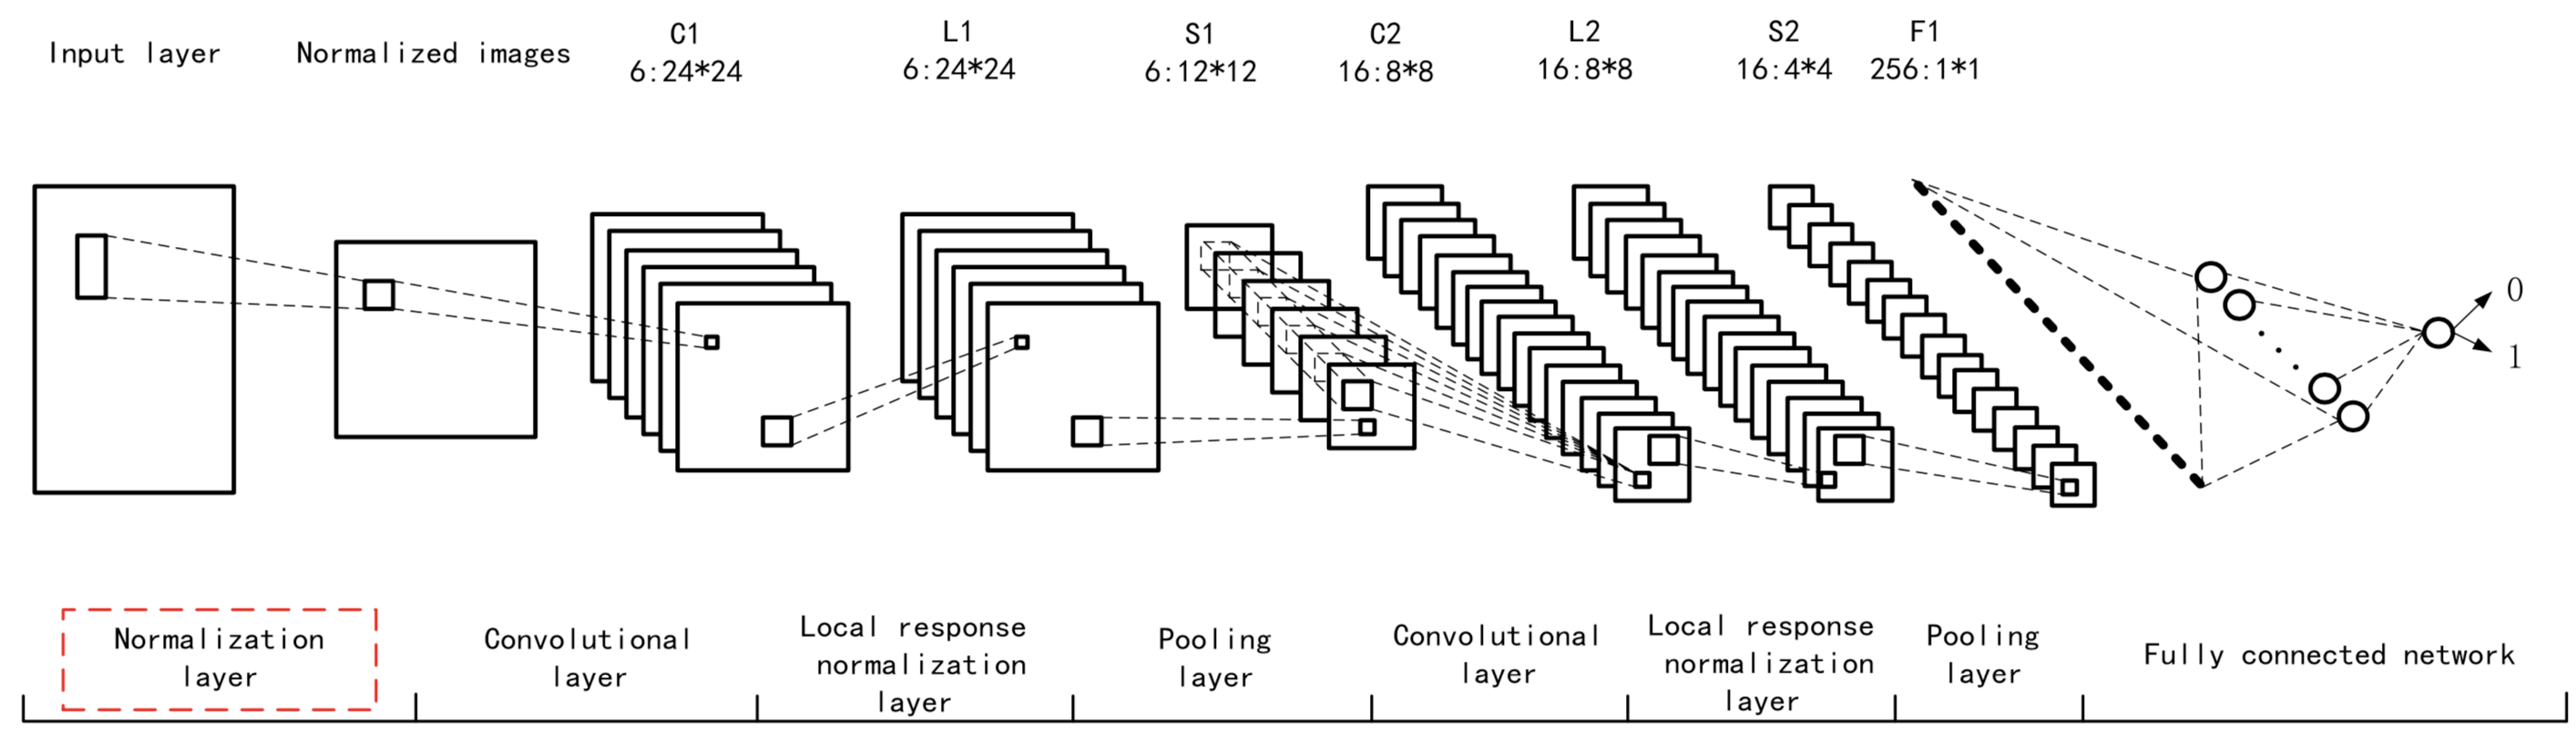
\includegraphics[scale=0.25]{pictures/CNN_feng2017.png}}
	\caption{Architecture of CNN from \cite{Feng2017}}
	\label{ris:CNN_feng2017}
\end{figure}
The interested reader can find all details and overall architecture parameters in \cite{Feng2017}.
From now on this CNN is marked as CNN-2 by the number of Convolutional layers.

We also reimplemented CNN from \cite{2020a}, which showed better results than pre-trained and fine-tuned OverFeatNet, VGGNet, GoogleNet networks.
The architecture is shown in Fig.~\ref{ris:raynet}.
Since our input size is smaller than in the original paper, we used smaller kernel size (3x3 instead of 7x7).
\begin{figure}[ht]
	\center{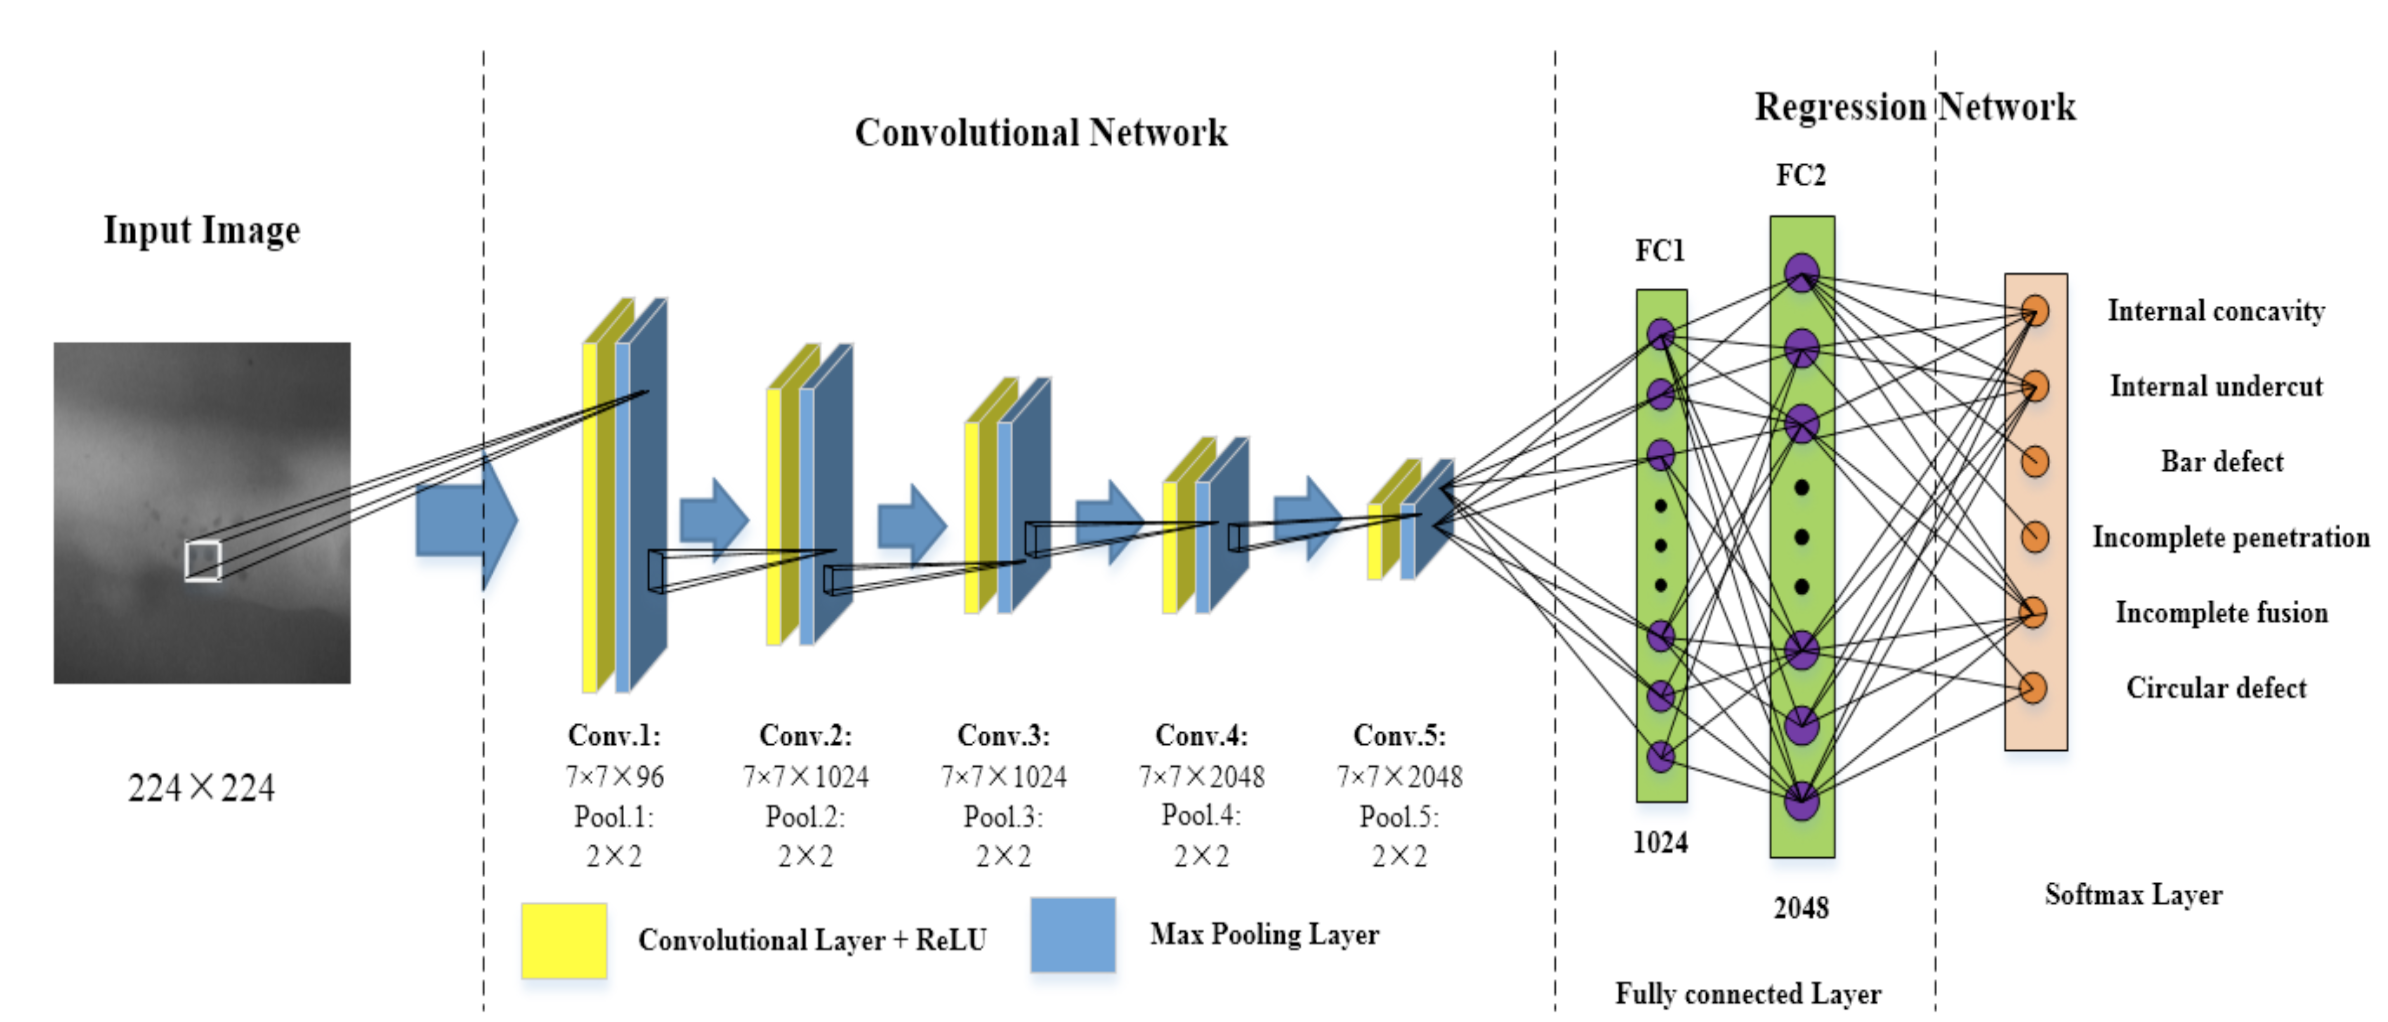
\includegraphics[scale=0.3]{pictures/raynet.png}}
	\caption{Architecture of CNN from \cite{2020a}}
	\label{ris:raynet}
\end{figure}
All details and CNN's parameters are presented in \cite{2020a}.
From now on this CNN is marked as RayNet.


\section{RESULTS}
\label{RESULTS}

We present the results of comparison for different preprocessing techniques and different CNN architectures for binary classification (normal pipe wall or defect/weld) in Tab.~\ref{tab:comp1} and multiclass classification problem (normal pipe wall, defect or weld) in Tab.~\ref{tab:comp2}.

Batch size is equal to 64, so the input to the network has shape (64, 1, 64, 64).
For all experiments, we use Adam optimizer with initial learning rate 0.001 and learning rate scheduler with parameters: threshold = 0.0001, factor = 0.5, min lr = 0.0001, patience = 484.
Also, for all experiments, the number of epochs is equal to 12.
Dropout rate for all experiments is equal to 0.33.
All mentioned parameters were selected by using grid search procedure.

\begin{table}[!htb]
	\caption{\label{tab:comp1}Comparison of performance among different classification methods for binary classification problem. $\hat{y}=y=0$ - healthy; $\hat{y}=y=1$ - defect/weld.}
	\begin{center}
		\small
		\begin{tabular}{| l | c | c | c |}
			\hline
			Method & $\hat{y}=y=0$ & $\hat{y}=y=1$ & Average \\
			\hline
			CNN-2 & 95.55 & 82.08 & 89.88 \\
			RayNet &  &  &  \\
			CNN-5 & 97.95 & \textbf{91.51} & \textbf{95.24} \\
			CNN-5+LRN & \textbf{98.29} & 89.86 & 94.74 \\
			\hline
			\multicolumn{4}{|c|}{Filling techniques comparison}  \\
			\hline
			CNN-5 (filling 1) & 97.95 & \textbf{91.51} & \textbf{95.24} \\
			CNN-5 (filling 2) & 97.95 & 84.20 & 92.16 \\
			CNN-5 (filling 3) & 97.26 & 83.02 & 91.27 \\
			CNN-5 (filling 4) & \textbf{98.63} & 81.13 & 91.27 \\
			CNN-5 (filling 5) & 98.12 & 81.84 & 91.27 \\
%			\hline
%			\multicolumn{4}{|c|}{Centering influence for the first filling method} \\
%			\hline
%			CNN-5 (centered) & 97.95 & \textbf{91.51} & 95.24 \\
%			CNN-5 (not centered) & \textbf{98.46} & 91.27 & \textbf{95.44} \\
%			CNN-2 (centered) & 95.55 & 82.08 & 89.88 \\
%			CNN-2 (not centered) & 96.92 & 80.42 & 89.81 \\
			\hline
		\end{tabular}
	\end{center}
\end{table}

Filling methods were researched for binary classification problem.
Centering means using peaks (extremums) searching procedure for welds or defects correct coordinates defining.
The centering procedure was research both for binary and multiclass classification problems.
Moreover, Min-Max normalization with using either a single image or whole dataset was investigated.
Finally, CNN-2 and CNN-5 were compared for centered images with the first filling method using single image Min-Max normalization.

\begin{table}[!htb]
	\caption{\label{tab:comp2}Comparison of performance among different classification methods for multiclass classification problem. $\hat{y}=y=0$ - healthy; $\hat{y}=y=1$ - defect; $\hat{y}=y=2$ - weld.}
	\begin{center}
		\small
		\begin{tabular}{| l | c | c | c | c |}
			\hline
			Method & $\hat{y}=y=0$ & $\hat{y}=y=1$ & $\hat{y}=y=2$ & Average \\
			\hline
			CNN-2 & 97.60 & 59.86 & 92.91 & 90.97 \\
			RayNet &  &  &  &  \\
			CNN-5 & \textbf{98.12} & \textbf{76.76} & \textbf{98.23} & \textbf{95.14} \\
%			\hline
%			\multicolumn{5}{|c|}{Centering influence for the first filling method}  \\
%			\hline
%			CNN-5 (centered) & \textbf{98.12} & \textbf{85.21} & 75.18 & 89.88 \\
%			CNN-5 (not centered) &  \textbf{98.12} & 76.76 & \textbf{98.23} & \textbf{95.14} \\
%			CNN-2 (centered) & 96.75 & 71.13 & 52.13 & 80.65 \\
%			CNN-2 (not centered) & 97.60 & 59.86 & 92.91 & 90.97 \\
			\hline
			\multicolumn{5}{|c|}{Single image normalization vs Whole dataset normalization}  \\
			\hline
			CNN-5 (1) (whole) & 97.95 & 64.08 & \textbf{99.65} & 93.65 \\
			CNN-5 (1) (image) &  98.12 & \textbf{76.76} & 98.23 & \textbf{95.14} \\
			CNN-2 (1) (whole) & \textbf{99.32} & 13.38 & 96.45 & 86.41 \\
			CNN-2 (1) (image) & 97.60 & 59.86 & 92.91 & 90.97 \\
			CNN-5 (3) (whole) & 99.66 & 81.69 & 99.65 & 97.12 \\
%			CNN-5 (3) (image) &  98.12 & \textbf{76.76} & 98.23 & \textbf{95.14} \\
			CNN-2 (3) (whole) & 95.72 & 13.38 & 97.52 & 89.58 \\
%			CNN-2 (3) (image) & 97.60 & 59.86 & 92.91 & 90.97 \\
			\hline
		\end{tabular}
	\end{center}
\end{table}

\section{CONCLUSION}
\label{CONCLUSION}
%TODO magnetographic image
Today, manual analysis of a magnetographic image is a bottleneck for the diagnosis of pipeline transport, since it costs a lot of money and is limited by human resources. This study allows us to hope that this process can be fully automated, which is likely to make the analysis more reliable, faster and cheaper.

%Insulators and oil pipelines are known to be an important component of the energy transmission systems. Yet on the other hand they are exposed to electrical, mechanical, and environmental stresses leading to different kind of defection. In this study, we focused on investigating approaches based on the deep learning techniques to detect and classify defected insulators and detect the defects in pipelines. In doing so, we utilized state-of-art CNNs such as UNets and VGG modified to match the task in hand. Multiple improvement of the existing literature were offered in this project. In spite of the previous works in the literature which were focused on a particular failure mode or defect of insulators, we had three different defects namely, insulators with: broken, burned and missing cap. The results showed successful performance of the trained UNet in segmentation task of insulators and the trained VGG as the second stage network in reaching a proper accuracy while classifying insulators into the possible considered classes. 
Also, the network (CNN-5) that outperformed currently used CNNs for defect detection of pipelines was proposed. Moreover, we proposed a modified UNet for defects of pipelines segmentation. The results of segmentation show the applicability of the proposed UNet for the size of defects evaluation. The results of the experiments prove that all parts of the oil pipeline diagnostics process can be fully automated with high quality.

Finally, there can be defined several project development options:
\begin{enumerate}
	\item better preprocessing, including manual pictures selection;
	\item multiclass defects classification;
	\item defected welds detection;
	\item applying some common archictures like VGG or ResNet;
	\item adding layers to the last Convolutional layer for defect depth evaluation;
	\item investigate the repeatability of the results for different datasets;
	\item using separate dataset for results evaluation.
\end{enumerate}


%% The Appendices part is started with the command \appendix;
%% appendix sections are then done as normal sections
%% \appendix

%% \section{}
%% \label{}

%% If you have bibdatabase file and want bibtex to generate the
%% bibitems, please use
%%
\bibliographystyle{elsarticle-num} 
\bibliography{biblio}

%% else use the following coding to input the bibitems directly in the
%% TeX file.

%\begin{thebibliography}{00}
%
%%% \bibitem{label}
%%% Text of bibliographic item
%
%\bibitem{}
%
%\end{thebibliography}
\end{document}
\endinput
%%
%% End of file `elsarticle-template-num.tex'.
